\chapter{Analisis}
\section{Arsitektur Perangkat Lunak}
Pada penelitian ilmiah ini akan dibangun sebuah perangkat lunak yang bertujuan membantu penggunanya untuk memprediksi kemacetan di kota Bandung. Perangkat lunak ini terdiri dari 3 lapisan utama: Lapisan pertama berfungsi mendengarkan \textit{tweets} yang telah disaring dan berasal dari Twitter \textit{streaming}. Lapisan kedua adalah pra-proses data agar \textit{tweets} yang telah disaring dirubah menjadi bahan pembelajaran JST yang terstruktur dengan baik, pada lapisan ini dibutuhkan interaksi manusia. Pada lapisan ketiga dalam perangkat lunak ini berfungsi memprediksi kemacetan berdasarkan nama jalan dan waktu. Arsitekturnya dapat dilihat pada gambar \ref{fig:arsitekturpl}
\begin{figure}
\centering
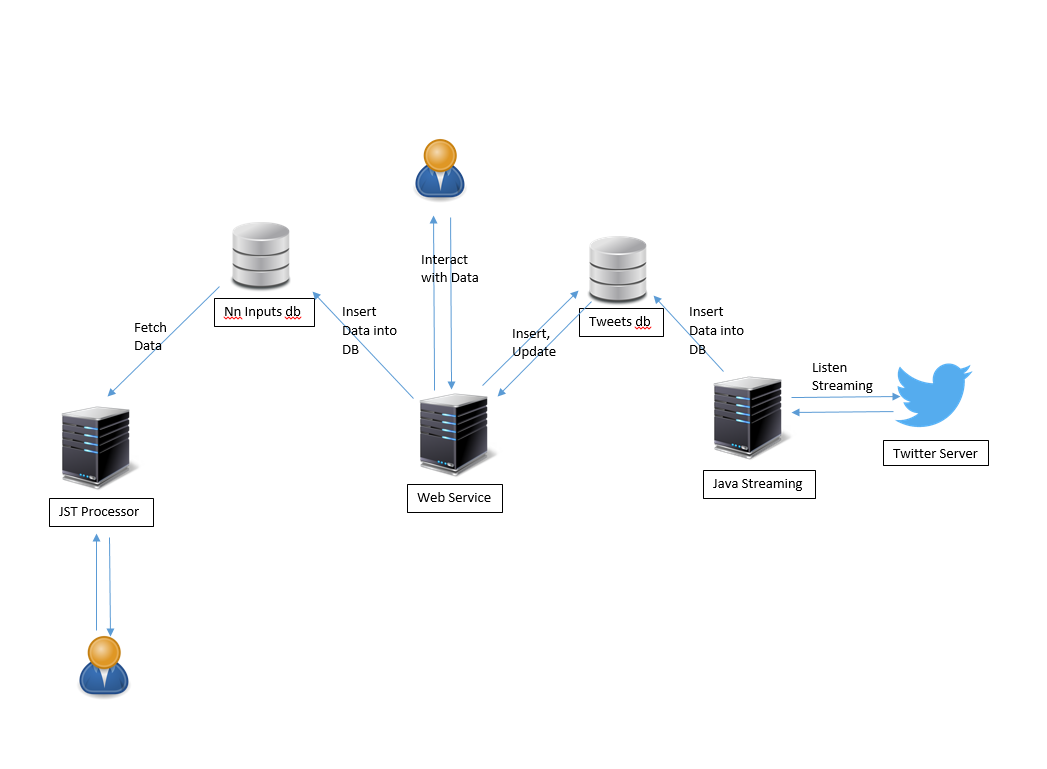
\includegraphics[width=0.6\linewidth]{Gambar/mine/sistem}
\caption[Arsitektur Perangkat Lunak]{Arsitektur Perangkat Lunak} 
\label{fig:arsitekturpl}
\end{figure}
\section{REST API atau Streaming API}
Pada lapisan pertama arsitektur digunakan untuk menarik \textit{tweets} yang berasal dari Twitter. Untuk menarik \textit{tweets} dari Twitter kedalam perangkat lunak akan digunakan \textit{library} Java bernama Twitter4j, library ini telah membungkus Twitter API agar dapat diimplementasikan kedalam pemograman bahasa Java. Pada bab dasar teori membahas bahwa Twitter API memiliki 2 cara dalam penarikan data yaitu REST API dan Streaming API. Bila kita teliti pada kebutuhan perangkat lunak, diperlukan jumlah data yang tidak sedikit untuk melakukan pemrosesan data pada arsitektur lapisan ketiga, maka harus dipilih jenis Twitter API yang dapat mengambil data secara berkala. Jika kita melihat salah satu API Twitter, REST API memiliki \textit{rate limits} yang membatasi perangkat lunak hanya dapat memanggil 180 perintah setiap 15 menit, karena batasan ini ada kemungkinan \textit{tweets} yang berharga dapat terlewat bahkan terjadi duplikasi \textit{tweets}. Berbeda seperti REST API, Streaming API tidak memiliki batasan untuk melakukan \textit{listen} pada server Twitter, dengan hal ini dapat memudahkan perangkat lunak dalam mengambil \textit{tweets} yang berlalu lalang di Server Twitter. Oleh karena itu perangkat lunak akan menggunakan Streaming API yang telah dibungkus oleh Twitter4j.
\section{Jenis Jaringan Syaraf Tiruan}
Tujuan penelitian ini adalah membangun perangkat lunak yang dapat memprediksi kemacetan. Jaringan Syaraf Tiruan adalah salah satu teknik yang tepat untuk memprediksi suatu kejadian berdasarkan kejadian-kejadian yang terjadi sebelumnya. Salah satu jenis JST yang popular dan sering digunakan untuk memprediksi ialah \textit{Feed Forward}. Untuk menggunakan JST \textit{Feed Foward} ada beberapa hal yang perlu ditentukan agar JST \textit{Feed Foward} dapat bekerja secara optimal, hal yang perlu ditentukan antar lain :
\begin{enumerate}
	\item Jumlah Hidden Layer dan Neuron setiap \textit{layer}
	\item Fungsi Aktivasi
	\item Metode Pembelajaran JST
\end{enumerate}
\subsection{Jumlah Hidden Layer dan Neuron setiap \textit{layer}}
Pada JST \textit{Feed Forward} terdiri 3 jenis \textit{layer}, \textit{input layer}, \textit{hidden layer}, \textit{output layer}. Setiap \textit{layer} terdiri dari neuron-neuron. Jumlah neuron ini perlu ditentukan,hal ini bergantung pada masalah dan keperluan JST. Dalam sub-bab ini peneliti akan menganalisis jumlah neuron setiap \textit{layer}-nya berdasarkan teknik yang telah dipaparkan pada bab-2. \\
Sebelum menentukan jumlah neuron setiap \textit{layer} pertama yang akan kita akan menentukan jumlah \textit{hidden layer}. Jumlah \textit{hidden layer} akan menentukan fungsi dari JST itu sendiri. Kita dapat melihat kembali pada tabel \ref{table:jmlhHiddenLayer} untuk menentukan jumlah hidden layer berdasarkan kegunaanya. Dapat hal memprediksi kemacetan dapat dimodelkan sebagai fungsi yang mengandung pemetaan kontinu. Oleh karena itu dengan hanya menggunakan satu buah hidden layer sudah cukup agar JST dapat memodelkan fungsi prediksi kemacetan.\\\\
Setelah menentukan jumlah \textit{hidden layer} kita akan menentukan jumlah neuron dalam \textit{input neuron}. Jumlah neuron pada \textit{input layer} bergantung pada data yang kita miliki, dan parameter apa saja yang diperlukan untuk melatih JST. Jika kita meninjau struktur data pelatihan terdiri dari hari, jam, nama lokasi, dan status kemacetan. Oleh karena itu jumlah neuron dalam \textit{hidden layer} akan berjumlah 4 buah.\\\\
Sama seperti \textit{input layer}, \textit{output layer} ditentukan berdasarkan kebutuhan. Karena \textit{output layer} berfungsi menentukan output tersebut berstatus macet atau tidak, makan jumlah neuron dalam output layer akan memiliki 2 buah neuron. Dimana setiap neuron akan merepresentasikan status dari kemacetan.\\\\
Berbeda dengan menentukan \textit{input} dan textit{output layer} tidak ada cara baku untuk menentukan jumlah \textit{hidden layer} namun ada teknik-teknik yang membantu kita menentukan jumlah \textit{hidden layer}. Pada bab-2 telah dipaparkan jumlah neuron harus berada diantara jumlah masukan dan keluaran. Jumlah neuron seharusnya 2/3 ukuran dari layer masukan, ditambah dengan layer keluaran. Ketiga jumlah neuron seharusnya kurang dari dua kali dari layer masukan. Bila menggunakan teknik tersebut jumlah neuron pada \textit{hidden layer} berjumlah 4 neuron.
\subsection{Fungsi Aktivasi}
Dalam bab-2 dipaparkan bahwa fungsi aktivasi dapat kita buat dan tentukan berdasarkan kebutuhan. Namun keluaran yang dihasilkan JST hanya akan menentukan apakah prediksi tersebut macet atau tidak, \textit{range} angka nol sampai satu sudah dapat merepresentasikan apakah keluaran bernilai macet atau tidak. Karena \textit{range}nya bernilai nol sampai satu, kita dapat menggunakan fungsi aktivasi yang sering digunakan yaitu sigmoid. Fungsi aktivasi sigmoid hanya akan menghasilkan nilai nol sampai dengan satu dapat kita lihat pada gambar \ref{fig:k_sigmoid} pemetaan fungsi sigmoid.
\subsection{Metode Pembelajaran}
\section{Pengumpulan data pelatihan JST}
Agar JST dapat memprediksi kemacetan dengan tepat, maka JST perlu dilatih dilakukan pembelajaran. Karena JST perlu belajar maka dibutuhkanya kumpulan data pelatihan. Data yang digunakan untuk memprediksi ialah data kejadian yang pernah terjadi di masa lalu. Data pelatihan ialah \textit{tweets} yang bersumber dari media sosial Twitter yang akan diambil oleh sistem secara kontinu. \textit{Tweets} yang akan dijadikan metode pelatihan akan disaring berdasarkan \textit{query} tertentu. Kriteria dibawah akan menjadi penyaring jenis \textit{tweets} apa yang akan diambil sebagai pra-data pelatihan.
\begin{enumerate}
	\item Pemilihan Nama Jalan
	\item Pemilihan Sumber \textit{tweets}
	\item Bahasa
\end{enumerate}
\subsection{Pra-proses input JST}
Setelah kita melakukan penyaringan terhadap \textit{tweets}, agar menjadi data pelatihan bagi JST kita harus melakukan pra-proses agar \textit{tweets} menjadi masukan yang dapat diterima bagi JST. Cara yang kita gunakan memprosesnya dengan cara manual yang menggunakan manusia untuk memparsing \textit{tweets} menjadi input JST. Pertama manusia akan memilih apakah \textit{tweets} memenuhi kriteria sebagai input JST. Kedua \textit{tweets} yang memenuhi kriteria akan di pra-proses informasi apa yang terdapat dari \textit{tweets}, jalan apa subjectnya dan keterangan dari kondisi jalan.\\\\
Selain memecah \textit{tweets} menjadi input yang dapat diterima JST. Input yang masuk kedalam JST harus memiliki nilai float antara nol sampai satu. Karena data dari tweets ada yang bertipe string, dan integer lebih besar dari 1. Nilai-nilai tersebut harus dinormalisasi agar bernilai antara nol sampai satu. Untuk setiap nilai metode normalisasinya akan berbeda. Hal yang akan dinormalisasi sebagai berikut :
\begin{enumerate}
	\item Hari
	\item Jam
	\item Status kemacetan
\end{enumerate}
\section{Rancangan Basis Data}
Perangkat lunak ini memerlukan sebuah tempat penyimpanan. Salah satu tempat penyimpanan yang populer dan mudah diimplementasikan kedalam berbagai bahasa ialah mysql. Mysql ialah salah satu basis data yang menggunakan sql sebagai bahasa untuk melakukan perintah. Perangkat lunak akan menyimpan \textit{tweets} yang disaring  dan juga menyimpan data pelatihan yang sudah dilakukan pra-proses. Rancangan basis data yang dibuat dapat dilihat pada gambar \ref{fig:r_table}
\begin{figure}
	\centering
	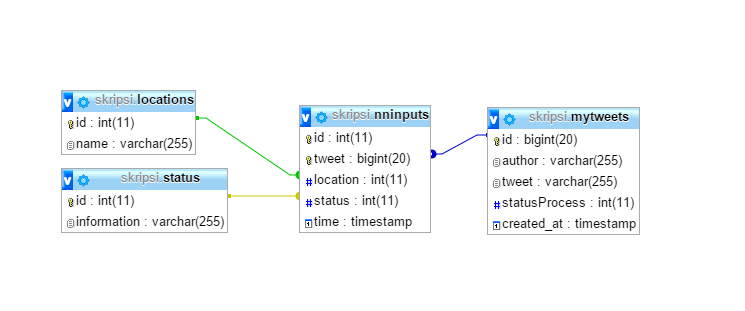
\includegraphics[width=1\linewidth]{Gambar/mine/relationalPL}
	\caption[Tabel Relational,]{Tabel Relational} 
	\label{fig:r_table}
\end{figure}